\documentclass[tikz, border=8pt]{standalone}
\usepackage{amsmath, bm}
\usetikzlibrary{calc, positioning, arrows.meta, backgrounds}

\definecolor{ink}{HTML}{1C1C1E}
\definecolor{inkgray}{HTML}{6E6E73}
\definecolor{buscol}{HTML}{824B50}
\definecolor{attnblue}{HTML}{C8DCF5}
\definecolor{moegreen}{HTML}{CBE7CF}
\definecolor{mlared}{HTML}{E6B3B2}
\definecolor{grayfill}{HTML}{F3F3F4}
\definecolor{salmonfill}{HTML}{F6D3CE}
\definecolor{gatefill}{HTML}{F2F3C1}

\pagecolor{white}
\begin{document}
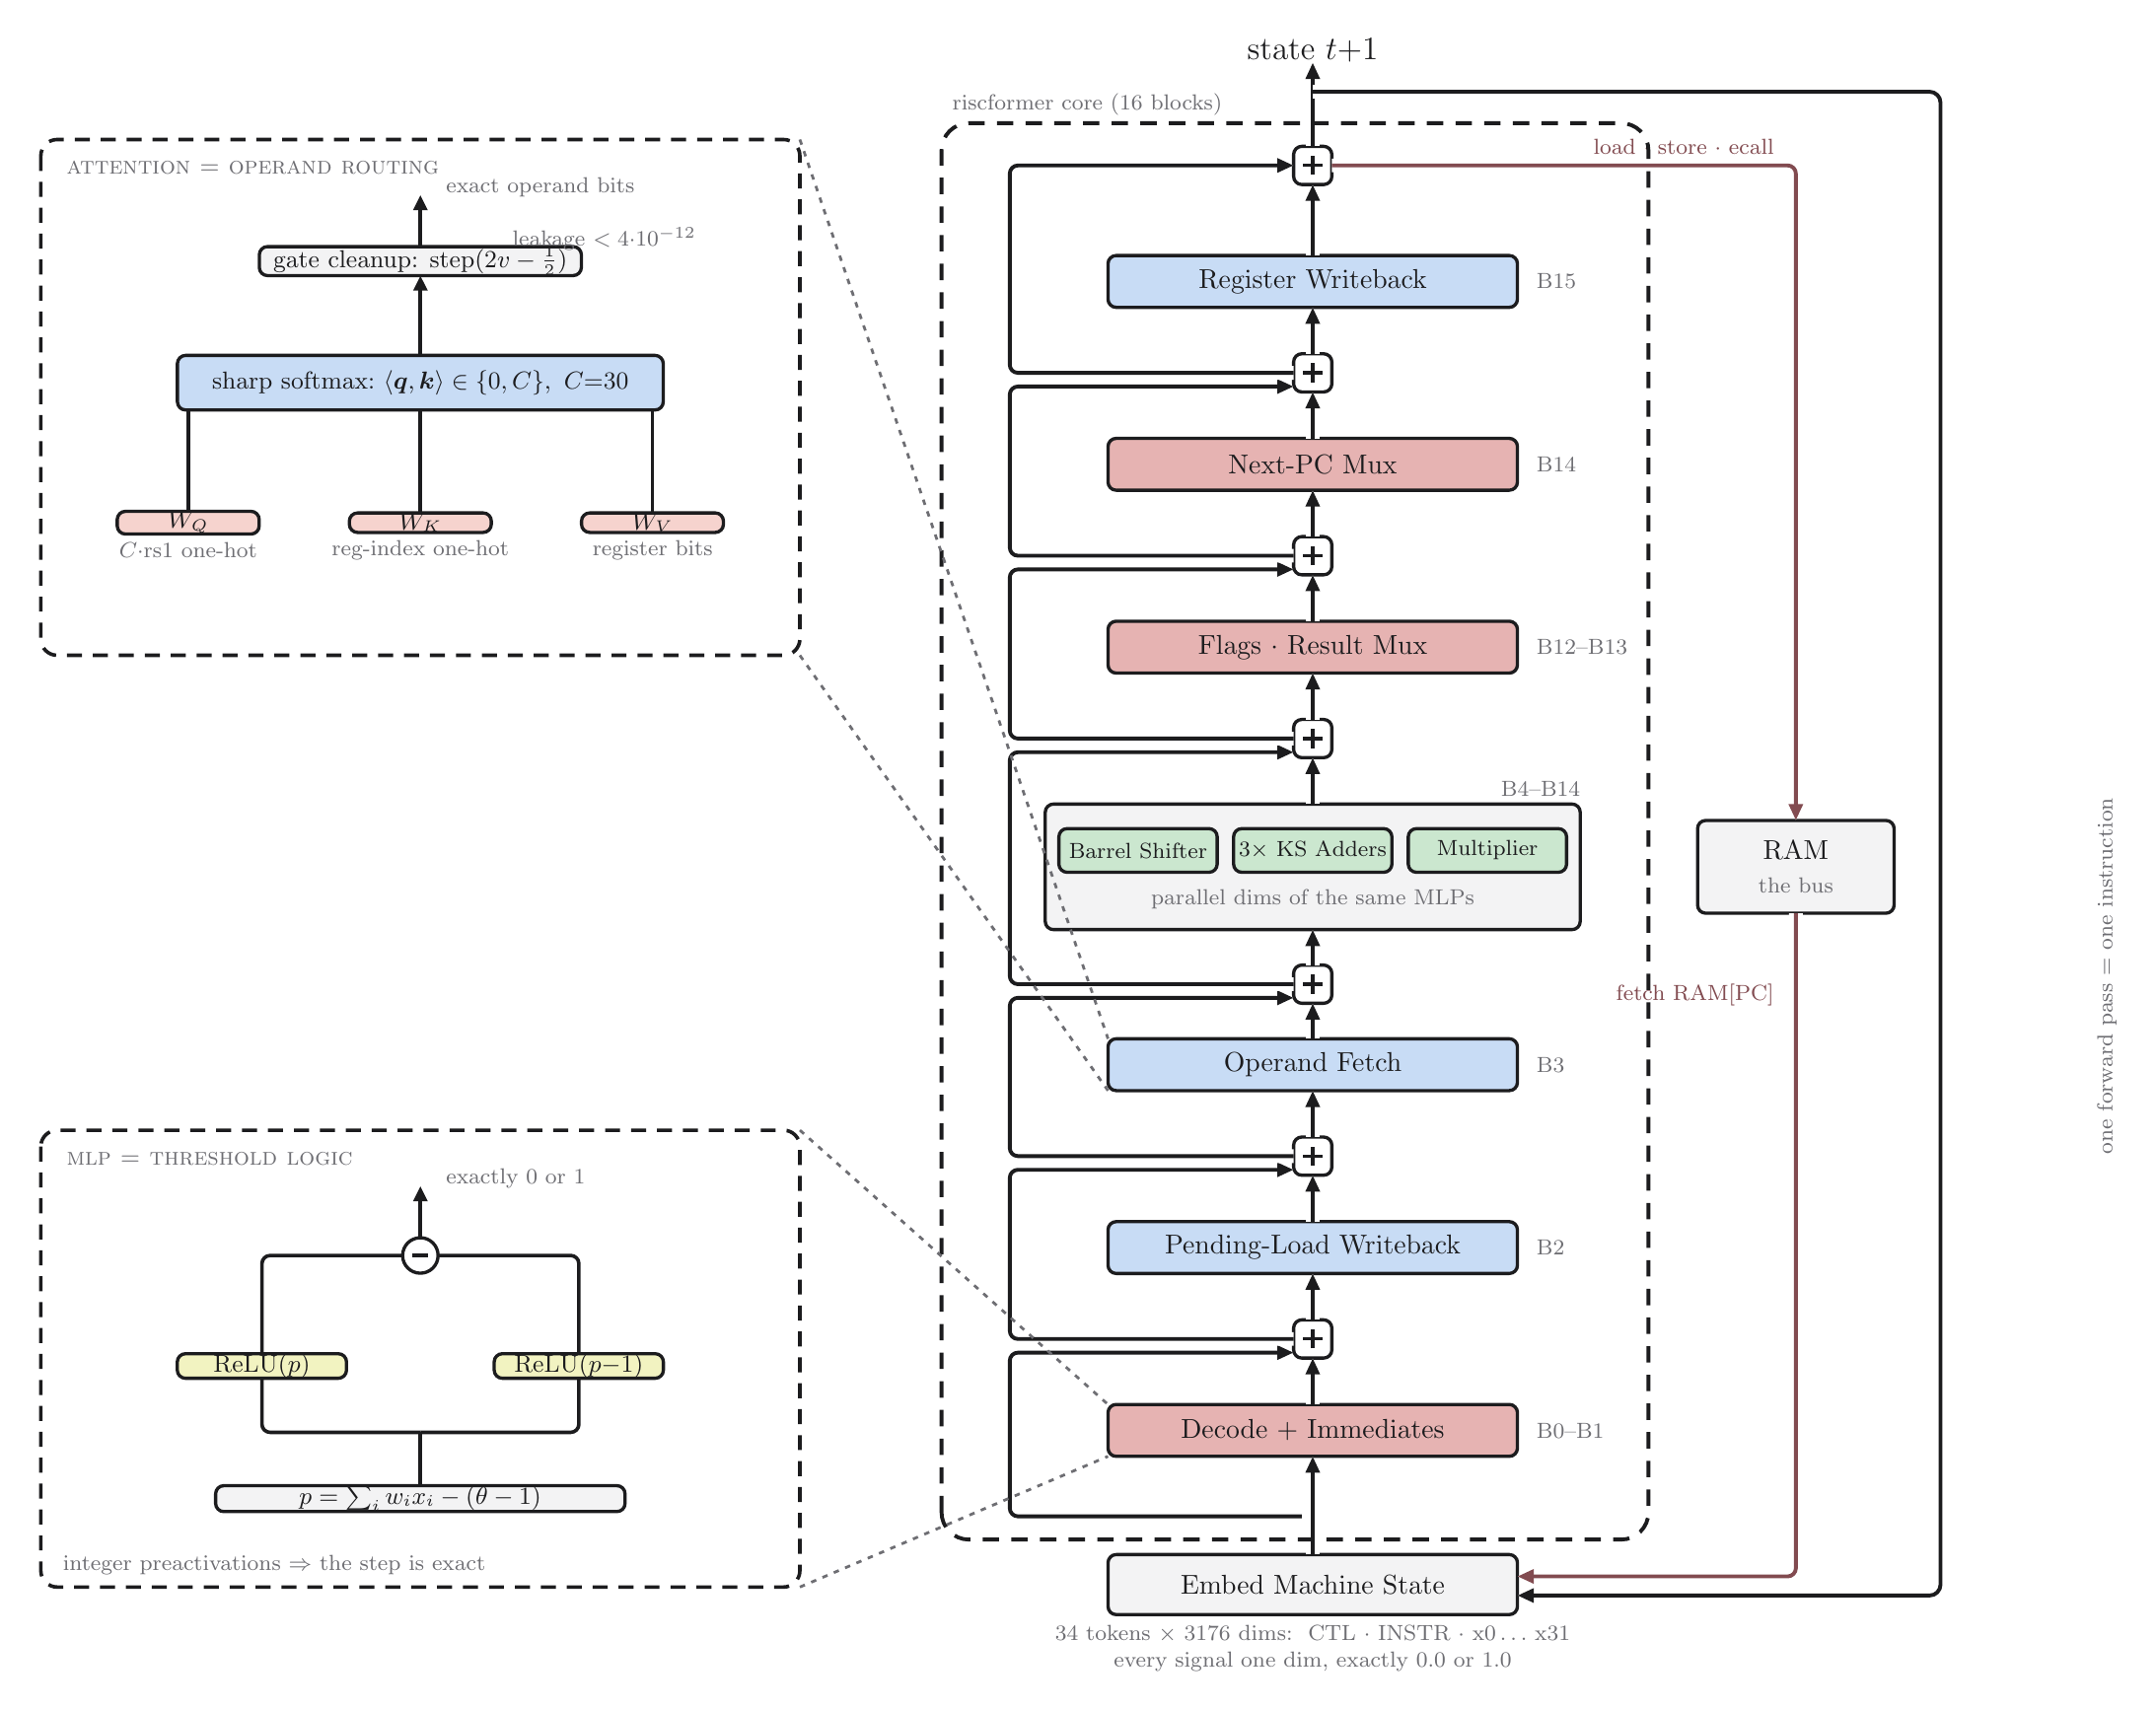
\begin{tikzpicture}[x=1pt, y=1pt, outer sep=0pt,
    show background rectangle,
    background rectangle/.style={fill=white},
    t12/.style={inner sep=0pt, text=ink, font=\large},
    t11/.style={inner sep=0pt, text=ink, font=\normalsize},
    t9/.style={inner sep=0pt, text=ink, font=\small},
    t8/.style={inner sep=0pt, text=inkgray, font=\footnotesize},
    arr/.style={-{Triangle[length=6pt,width=5pt]}},
    arrS/.style={-{Triangle[length=5.5pt,width=5pt]}},
    halo/.style={preaction={draw=white, line width=5pt, line join=round}},
    wire/.style={halo, draw=ink, line width=1.4pt, line join=round},
    flow/.style={wire, arr},
    bus/.style={halo, draw=buscol, line width=1.4pt, line join=round},
    busarr/.style={bus, arr},
    wireS/.style={draw=ink, line width=1.3pt, line join=round},
    flowS/.style={wireS, arrS},
    zoom/.style={draw=inkgray, line width=1pt, dash pattern=on 2pt off 2.5pt},
    module/.style={draw=ink, fill=#1, line width=1.2pt, rounded corners=3pt,
                   minimum width=150pt, minimum height=19pt, inner sep=0pt, t11},
    halfmod/.style={draw=ink, fill=#1, line width=1.2pt, rounded corners=3pt,
                   minimum width=71pt, minimum height=19pt, inner sep=0pt, t9},
    oplus/.style={draw=ink, fill=white, line width=1.2pt, rounded corners=3pt,
                  minimum width=14pt, minimum height=14pt, inner sep=0pt,
                  path picture={\draw[ink, line width=1.2pt]
                    ($(path picture bounding box.center)+(-3.5pt,0)$) -- ++(7pt,0)
                    ($(path picture bounding box.center)+(0,-3.5pt)$) -- ++(0,7pt);}},
    ominus/.style={draw=ink, fill=white, line width=1.2pt, circle, minimum size=13pt,
                  inner sep=0pt,
                  path picture={\draw[ink, line width=1.2pt]
                    ($(path picture bounding box.center)+(-3pt,0)$) -- ++(6pt,0);}},
    chip/.style={draw=ink, fill=grayfill, line width=1.2pt, rounded corners=3pt,
                 minimum width=150pt, minimum height=22pt, inner sep=0pt, t11},
    ramchip/.style={draw=ink, fill=grayfill, line width=1.2pt, rounded corners=3pt,
                 minimum width=72pt, minimum height=34pt, inner sep=0pt, t11},
    mainframe/.style={draw=ink, line width=1.4pt, dash pattern=on 6pt off 4.5pt,
                      rounded corners=10pt},
    pbox/.style={draw=ink, fill=#1, line width=1.2pt, rounded corners=3pt, inner sep=2.5pt, t9},
    pframe/.style={draw=ink, line width=1.3pt, dash pattern=on 5.5pt off 4pt,
                   rounded corners=6pt},
  ]

  % ============================ main stack ============================
  \node[module=mlared] (dec) at (340,-40) {Decode $+$ Immediates};
  \node[module=attnblue, above=48pt of dec] (pwb) {Pending-Load Writeback};
  \node[module=attnblue, above=48pt of pwb] (opf) {Operand Fetch};
  \node[draw=ink, fill=grayfill, line width=1.2pt, rounded corners=3pt,
        minimum width=196pt, minimum height=46pt, inner sep=0pt,
        above=40pt of opf] (exec) {};
  \node[pbox=moegreen, minimum width=58pt, minimum height=16pt]
        at ($(exec.center)+(-64pt,6pt)$) {\footnotesize Barrel Shifter};
  \node[pbox=moegreen, minimum width=58pt, minimum height=16pt]
        at ($(exec.center)+(0pt,6pt)$) {\footnotesize $3\times$ KS Adders};
  \node[pbox=moegreen, minimum width=58pt, minimum height=16pt]
        at ($(exec.center)+(64pt,6pt)$) {\footnotesize Multiplier};
  \node[t8] at ($(exec.center)+(0,-12pt)$)
        {parallel dims of the same MLPs};
  \coordinate (exe) at (exec.north);
  \coordinate (exes) at (exec.south);
  \node[module=mlared] (res) at ($(dec)+(0,287pt)$) {Flags $\cdot$ Result Mux};
  \node[module=mlared, above=48pt of res] (npc) {Next-PC Mux};
  \node[module=attnblue, above=48pt of npc] (rwb) {Register Writeback};

  % residual adds between stages
  \foreach \a/\b/\p in {dec/pwb/p1, pwb/opf/p2, res/npc/p5, npc/rwb/p6}
    \node[oplus] (\p) at ($(\a.north)!0.5!(\b.south)$) {};
  \node[oplus] (p3) at ($(opf.north)!0.5!(exes)$) {};
  \node[oplus] (p4) at ($(exe)!0.5!(res.south)$) {};
  \node[oplus, above=26pt of rwb] (p7) {};

  % embedding chip
  \node[chip, below=36pt of dec] (emb) {Embed Machine State};
  \node[t8, below=4pt of emb, align=center]
    {34 tokens $\times$ 3176 dims:\ \ CTL $\cdot$ INSTR $\cdot$ x0\,\dots\,x31\\
     every signal one dim, exactly $0.0$ or $1.0$};

  % residual skip wires: exit each join's west, re-enter the next join low-west
  \coordinate (bin) at ($(emb.north)+(0,14pt)$);
  \draw[flow, rounded corners=3pt] ($(bin)+(-4pt,0)$) -- ++(-107pt,0) |- ([yshift=-5pt]p1.west);
  \foreach \p/\q in {p1/p2, p2/p3, p3/p4, p4/p5, p5/p6}
    \draw[flow, rounded corners=3pt] (\p.west) -- ++(-104pt,0) |- ([yshift=-5pt]\q.west);
  \draw[flow, rounded corners=3pt] (p6.west) -- ++(-104pt,0) |- (p7.west);

  % vertical flow
  \draw[flow] (dec.north) -- (p1.south);
  \draw[flow] (p1.north) -- (pwb.south);
  \draw[flow] (pwb.north) -- (p2.south);
  \draw[flow] (p2.north) -- (opf.south);
  \draw[flow] (opf.north) -- (p3.south);
  \draw[flow] (p3.north) -- (exec.south);
  \draw[flow] (exec.north) -- (p4.south);
  \draw[flow] (p4.north) -- (res.south);
  \draw[flow] (res.north) -- (p5.south);
  \draw[flow] (p5.north) -- (npc.south);
  \draw[flow] (npc.north) -- (p6.south);
  \draw[flow] (p6.north) -- (rwb.south);
  \draw[flow] (rwb.north) -- (p7.south);

  % block indices
  \foreach \m/\l in {dec/B0--B1, pwb/B2, opf/B3, res/B12--B13, npc/B14, rwb/B15}
    \node[t8, anchor=west] at ($(\m.east)+(7pt,0)$) {\l};
  \node[t8, anchor=south east] at ($(exec.north east)+(0pt,3pt)$) {B4--B14};

  \draw[flow] (emb.north) -- (dec.south);

  % output
  \node[t12] (out) at ($(p7)+(0,42pt)$) {state $t{+}1$};
  \draw[flow] (p7.north) -- (out.south);

  % ============================ RAM + recurrence ============================
  \node[ramchip, align=center] (ram) at ($(exec.east)+(79pt,0)$)
        {RAM\\{\footnotesize\textcolor{inkgray}{the bus}}};
  \draw[busarr, rounded corners=3pt] (ram.south) |- ($(emb.east)+(0,3pt)$);
  \node[t8, anchor=east, text=buscol] at ($(ram.south)+(-8pt,-30pt)$) {fetch RAM[PC]};
  \draw[busarr, rounded corners=3pt] (p7.east) -- (p7.east -| ram.north) -- (ram.north);
  \node[t8, anchor=south east, text=buscol] at ($(p7.east -| ram.north)+(-8pt,4pt)$) {load $\cdot$ store $\cdot$ ecall};
  % recurrence lane (outermost right)
  \coordinate (rtap) at ($(p7.north)+(0,20pt)$);
  \draw[flow, rounded corners=4pt] (rtap) -- ++(230pt,0) |- ($(emb.east)+(0,-4pt)$);
  \node[t8, rotate=90, anchor=center] at ($(ram.east)+(78pt,-40pt)$) {one forward pass $=$ one instruction};

  % main dashed frame
  \coordinate (frSW) at ($(dec.west)+(-61pt,-40pt)$);
  \coordinate (frNE) at ($(rwb.east)+(48pt,58pt)$);
  \draw[mainframe] (frSW) rectangle (frNE);
  \node[t8, anchor=south west] at ($(frSW |- frNE)+(4pt,3pt)$) {riscformer core (16 blocks)};

  % ============================ zoom panel A: attention ============================
  \begin{scope}[shift={($(frSW |- frNE)+(-330pt,-6pt)$)}, scale=1.35]
    \draw[pframe] (0,0) rectangle (206,-140);
    \coordinate (paNE) at (206,0);
    \coordinate (paSE) at (206,-140);
    \node[t9, anchor=north west, text=inkgray] at (7,-6) {\textsc{attention $=$ operand routing}};

    \node[pbox=salmonfill, minimum width=52pt] (wq) at (40,-104) {$W_Q$};
    \node[pbox=salmonfill, minimum width=52pt] (wk) at (103,-104) {$W_K$};
    \node[pbox=salmonfill, minimum width=52pt] (wv) at (166,-104) {$W_V$};
    \node[t8, below=3pt of wq] {$C\cdot$rs1 one-hot};
    \node[t8, below=3pt of wk] {reg-index one-hot};
    \node[t8, below=3pt of wv] {register bits};

    \node[pbox=attnblue, minimum width=178pt, minimum height=20pt] (smax) at (103,-66)
      {sharp softmax:\ $\langle\bm q,\bm k\rangle\in\{0,C\},\ C{=}30$};
    \node[pbox=grayfill, minimum width=118pt] (clean) at (103,-33)
      {gate cleanup: $\mathrm{step}(2v-\tfrac12)$};

    \foreach \w in {wq, wk, wv} \draw[wireS] (\w.north) -- (\w.north |- smax.south);
    \draw[flowS] (smax.north) -- (clean.south);
    \node[t8, anchor=south west] at (128,-30) {leakage $<4{\cdot}10^{-12}$};
    \draw[flowS] (clean.north) -- ++(0,14pt);
    \node[t8, anchor=west] at (110,-13) {exact operand bits};
  \end{scope}
  \draw[zoom] (paNE) -- (opf.north west);
  \draw[zoom] (paSE) -- (opf.south west);

  % ============================ zoom panel B: threshold gate ============================
  \begin{scope}[shift={($(frSW)+(-330pt,150pt)$)}, scale=1.35]
    \draw[pframe] (0,0) rectangle (206,-124);
    \coordinate (pbNE) at (206,0);
    \coordinate (pbSE) at (206,-124);
    \node[t9, anchor=north west, text=inkgray] at (7,-6) {\textsc{mlp $=$ threshold logic}};

    \node[pbox=grayfill, minimum width=150pt] (pre) at (103,-100)
      {$p=\textstyle\sum_i w_i x_i - (\theta - 1)$};
    \node[pbox=gatefill, minimum width=62pt] (r1) at (60,-64) {$\mathrm{ReLU}(p)$};
    \node[pbox=gatefill, minimum width=62pt] (r2) at (146,-64) {$\mathrm{ReLU}(p{-}1)$};
    \node[ominus] (sub) at (103,-34) {};
    \coordinate (pj) at (103,-82);
    \draw[wireS] (pre.north) -- (pj);
    \draw[wireS, rounded corners=3pt] (pj) -| (r1.south);
    \draw[wireS, rounded corners=3pt] (pj) -| (r2.south);
    \draw[wireS, rounded corners=3pt] (r1.north) |- ($(sub.west)+(-4pt,0)$) -- (sub.west);
    \draw[wireS, rounded corners=3pt] (r2.north) |- ($(sub.east)+(4pt,0)$) -- (sub.east);
    \draw[flowS] (sub.north) -- ++(0,14pt);
    \node[t8, anchor=west] at (110,-13) {exactly $0$ or $1$};
    \node[t8, anchor=west] at (6,-118) {integer preactivations $\Rightarrow$ the step is exact};
  \end{scope}
  \draw[zoom] (pbNE) -- (dec.north west);
  \draw[zoom] (pbSE) -- (dec.south west);

\end{tikzpicture}
\end{document}
